\documentclass[12pt]{article} 

\usepackage[utf8]{inputenc}
\usepackage[OT1]{fontenc}

% Gestion de la langue du document
\usepackage[french]{babel}

% Gestion des espaces
\usepackage{xspace}

% Gestion des images
\usepackage{graphicx}

% Pour permettre la redéfinition des dimensions
\usepackage[a4paper]{geometry}

%Gestion des images dans le document
\usepackage{subcaption}

%Gestion des lien hypertext
\usepackage{hyperref}

% Configuration des dimensions
\geometry{%
left=20mm,width=165mm,
top=15mm,height=267mm,
footskip=15mm}

% Le titre
\title{Rapport_TD_Outils-Libres}
\author{Enzo Collot}
\date{Année universitaire 2022-2023}


\begin{document}

    \thispagestyle{empty}
    \begin{center}
        
\includegraphics[width=12cm]{Image-TD-1/logo_iut.jpg}
        \end{center}

\vspace{1cm}

\noindent
{\large
  IUT Nancy Charlemagne\\
  Université de Lorraine\\
  2 ter boulevard Charlemagne\\
  BP 55227\\
  54052 Nancy Cedex\\[5mm]
  Département informatique
}

\vspace{5cm}

\begin{center}
    {\huge
      \textbf{Rapport TD Outils-Libres en Latex}
    }
\end{center}

\vspace{5cm}

% \vspace{2cm}
\vfill


{\Large
  \noindent
  Etudiant : Enzo Collot\\
  Année universitaire 2022--2023
}

% Ajout d'une page vide
\newpage
\thispagestyle{empty}
\mbox{}
\newpage

\newpage
% Table des matières
\tableofcontents

\newpage

\section{Efficacité de l'environnement de travail}

  \subsection{TD-1 : La souris}

\begin{itemize}
  \item Désactiver votre souris au niveau système avec la commande xinput
\end{itemize}

\vspace{0.3cm}

Pour désactiver la souris au niveau système, nous allons utiliser la commande \texttt{xinput}.

\vspace{0.3cm}

Je tiens à préciser que je vais effectuer ce test sur mon ordinateur personnel qui fonctionne sous Linux Mint.

\vspace{0.3cm}

Voici ci-dessous, la commande qui permet de désactiver la souris :

\begin{verbatim}
xinput set-prop "device name" "Device Enabled" 0
\end{verbatim}

Dans mon cas, j'ai dû rentrer la commande suivante :

\begin{verbatim}
xinput set-prop "Logitech Wireless Receiver Mouse" "Device Enabled" 1
\end{verbatim}

\vspace{0.3cm}

\begin{itemize}
  \item Initialiser un fichier dans lequel nous allons lister tous les problèmes d'efficacité rencontrés pendant cette séance.
\end{itemize}
\vspace{0.3cm}

\begin{tabular}{|c|p{5cm}|p{10cm}|}
  \hline
  \textbf{Priorité} & \textbf{Problème} & \textbf{Correctif}\\
  \hline 
  1 & Logout difficile au clavier & Raccourci clavier \textbf{Ctrl+Alt+Suppr/Delete}\\
  \hline
  2 & Impossible d'éditer des documents PDF avec Google Drive & Utilisation de LaTeX\\
  \hline
  3 & La souris est bloquée et ne répond plus & Utilisez le raccourci clavier \textbf{Ctrl+Alt+F1} pour ouvrir une console en mode texte, puis connectez-vous à votre session. Ensuite, utilisez la commande \textbf{sudo service gdm3 restart} pour redémarrer le serveur d'affichage et réinitialiser la souris \\
  \hline
  4 & Impossible d'avoir plusieurs terminaux en parallèle & Sous Terminator, \textbf{Ctrl+Shift+O} pour split le terminal verticalement,\newline \textbf{Ctrl+Shift+L} pour split le terminal horizontalement\\ 
  \hline
  5 & Accèder au navigateur de fichier & shotcut configurable dans les settings ex : \textbf{Alt+F}\\
  \hline
  6 & Naviguer dans discord sans la souris & \textbf{Tab} pour se déplacer de haut en bas, \textbf{Shift+Tab} pour aller de bas en haut \newline et \textbf{Ctrl+Tab} pour naviguer de gauche à droite\\
  \hline
  7 & La souris ne fonctionne pas sur un ordinateur portable & Utilisez le raccourci clavier \textbf{Fn+F9} pour activer ou désactiver le pavé tactile, qui peut parfois interférer avec la souris \\
  \hline

\end{tabular}

\newpage

  \subsection{TD-2 : Le clavier}

\begin{itemize}
  \item Identifier un site permettant de s'améliorer à taper au clavier.
\end{itemize}

\vspace{0.3cm}

J'ai trouvé un site qui permet de tester la rapidité de frappe au clavier. Voici le lien ci-dessous  : 

\href{https://www.taptouche.com/fr/test-de-vitesse}{Site de TapTouch}

\vspace{0.3cm}

Pourquoi celui-ci plutôt qu'un autre ?

\vspace{0.3cm}

J'ai choisie ce site car il explique quelques informations sur notre score à la fin et il nous donne des astuces pour nous améliorer.

\vspace{0.3cm}

Inclure quelques screenshots montrant l'interface

\vspace{0.3cm}

Screen de l'interface du site :

\vspace{0.3cm}

\begin{figure}[h]
  \centering
  \begin{subfigure}{0.45\textwidth}
    \centering
    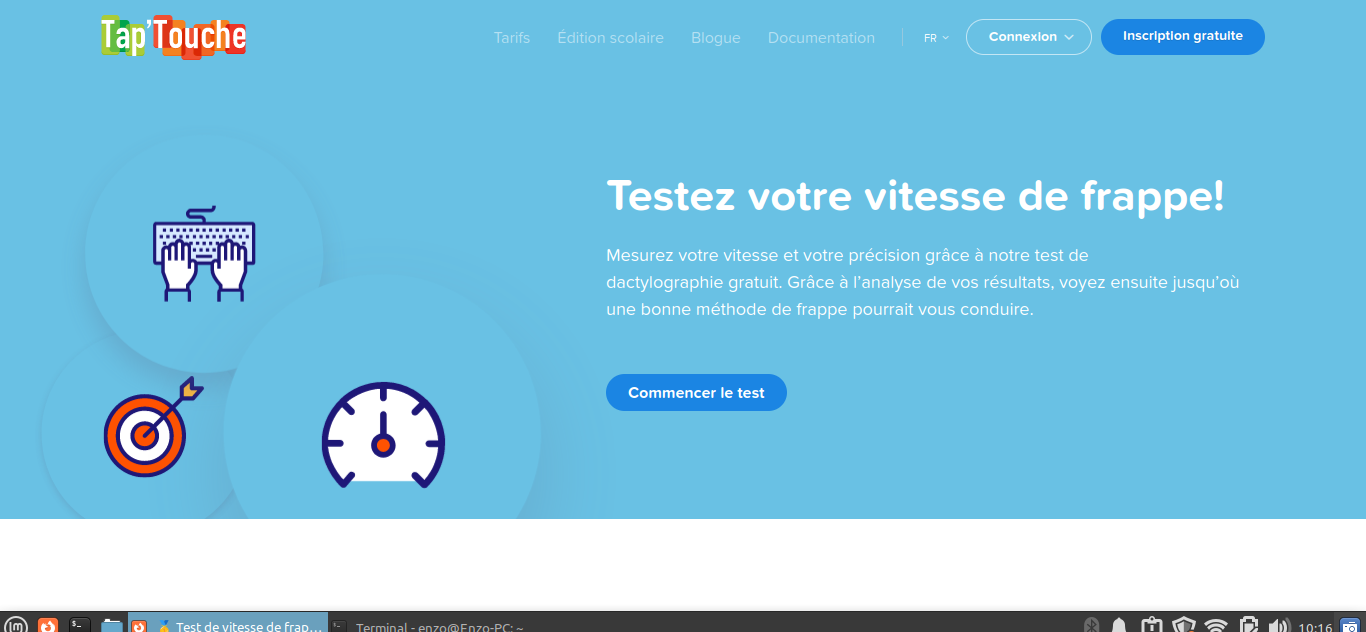
\includegraphics[width=\textwidth]{Image-TD-2/image_site_tap_touche.png}
    \caption{Page principale du site}
  \end{subfigure}
  \vspace{0.9cm} % Espace verticale entre les images
  \begin{subfigure}{0.45\textwidth}
    \centering
    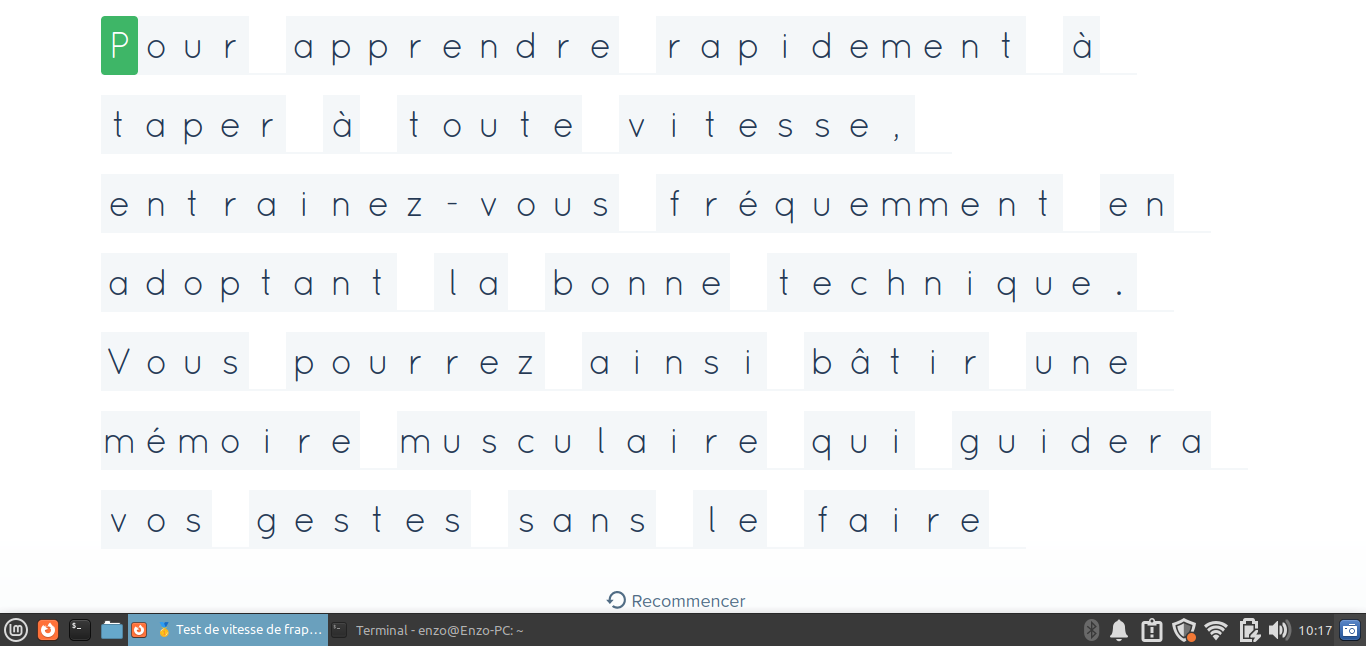
\includegraphics[width=\textwidth]{Image-TD-2/image_site_tap_touche2.png}
    \caption{Page pour effectuer le test de rapidité}
  \end{subfigure}
  \caption{Deux captures d'écran du site TapTouch}
\end{figure}

\vspace{0.3cm}

Essayer de masquer ses mains pour taper sans regarder

\vspace{0.3cm}

Inclure quelques résultats de rapidité.

\vspace{0.3cm}

Premier test effectué le 22/12/2022 : 

\begin{center}
  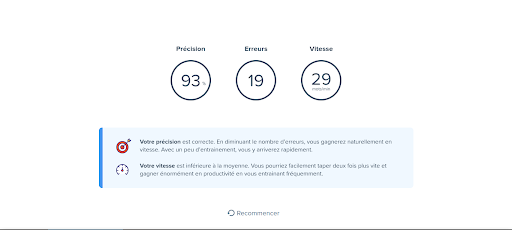
\includegraphics[width=10cm]{Image-TD-2/Premier_test.png}
\end{center}

\vspace{0.3cm}

\newpage

Deuxième test effectué le 23/12/2022 :

\begin{center}
  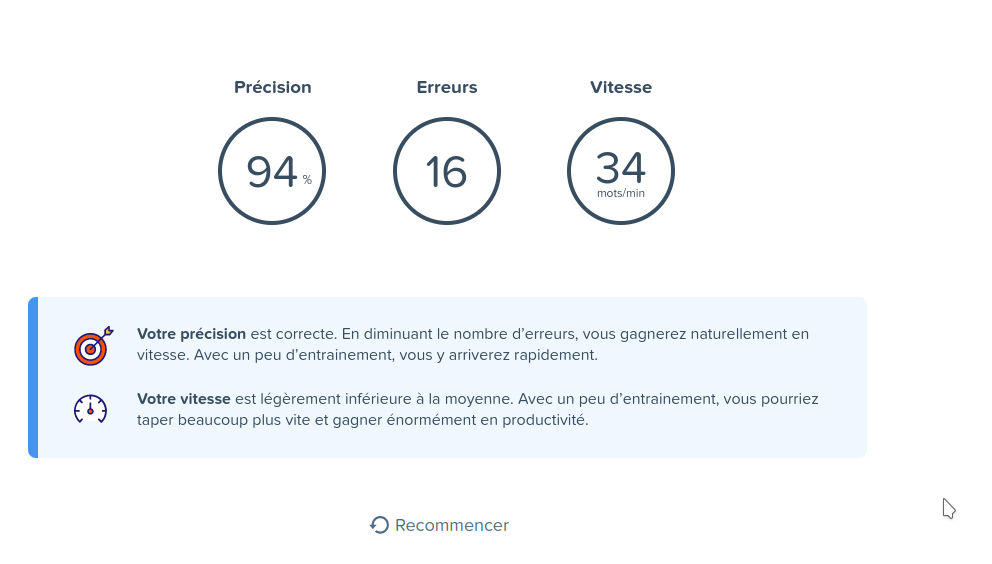
\includegraphics[width=10cm]{Image-TD-2/Deuxième_test.png}
\end{center}

\subsection{TD-3 : Vim et Emacs}

\begin{itemize}
  \item Effectuer les tutoriels pour Vim et Emacs :\\
  Vim : \texttt{vimtutor}\\
  Emacs : \texttt{emacs}, puis \texttt{Ctrl+H+T}
\end{itemize}

\vspace{0.3cm}

\begin{itemize}
  \item Paramétrer GNU Readline (le line editor par défault de bash) pour être en mode Emacs ou Vim
\end{itemize}

\vspace{0.3cm}

Une fois que j'ai effectué les deux tutoriels, je vais paramétrer GNU Readline en mode Vim. Pour ce faire, je vais utiliser la commande suivante :

\vspace{0.3cm}

\texttt{export EDITOR=vim}

\vspace{0.3cm}

Aprés, pour l'avoir de façon permanente, on peut ajouter cette ligne dans le fichier \texttt{~/.bashrc}.

\vspace{0.3cm}

\begin{itemize}
  \item Tester les deux 2 modes, en choisir un
\end{itemize}

\vspace{0.3cm}

J'ai testé ces deux modes et j'ai choisie d'utiliser Vim. 

\vspace{0.3cm}

\begin{itemize}
  \item Paramétrer Emacs ou Vim comme étant éditeur par défault en plus du mode Readline.
\end{itemize}

\vspace{0.3cm}

Pour qu'il soit de façon permanente, j'ai ajouté cette ligne suivante dans le fichier bashrc comme ci-dessous :

\vspace{0.3cm}

\begin{center}
  
\includegraphics[width=10cm]{Image-TD-3/Ajout-ligne-bashrc.png}
\end{center}

\newpage

  \subsection{TD-4 : Commande history}

\begin{itemize}
  \item Regarder votre history
\end{itemize}

\vspace{0.3cm}

Voici ci-dessous, une capture d'écran de mon history : 

\begin{center}
  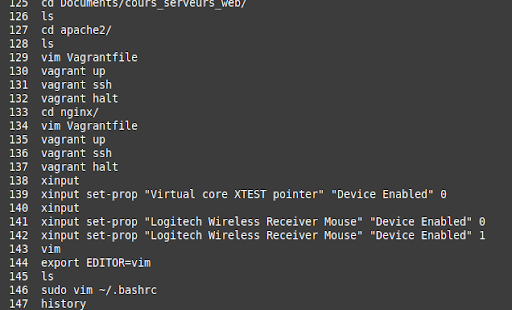
\includegraphics[width=10cm]{Image-TD-4/history.png}
\end{center}

\vspace{0.3cm}

\begin{itemize}
  \item Y a-t-il des informations sensible ? Comment y remédier ?
\end{itemize}

\vspace{0.3cm}

Oui, il peut y avoir des informations sensibles dans le history comme les mot de passe etc. Pour remédier à cela, nous pouvons utiliser un autre interpréteur de commande comme ZSH.

\vspace{0.3cm}

\begin{itemize}
  \item Un employé de longue date semble avoir un \texttt{history} très court, quelle sont les causes possibles ?\\
  \vspace{0.3cm}
  ~ cat ~/.bash\_history\\
  \vspace{0.3cm}
  sudo apt install curl zsh git\\
  \vspace{0.3cm}
  sh -c "(curl -fsSL https://raw.github.com/ohmyzsh/ohmyzsh/master/tools/install.sh)" 
\end{itemize}

\vspace{0.3cm}

On peut constater que cette employé à utiliser un autre interpréteur de commande qui est ZSH en le combinant avec OHMYZSH. Donc on ne peut plus voir son hisotry dans bash\_history.

\vspace{0.3cm}

\begin{itemize}
  \item Nos history sont souvent pollués par beaucoup de ls, cd, pwd ... Ces commandes sont tellement courtes que les taper entièrement est plus rapide. On veut éviter qu'elles n'apparaissent dans les résultats de recherche de l'history, comment faire ?
\end{itemize}

\vspace{0.3cm}

Pour eviter d'avoir certaine commande dans notre hisotry, on peut ajouter l'option \texttt{HISTIGNORE} dans le fichier bashrc : 

\vspace{0.3cm}

\begin{center}
  
\includegraphics[width=10cm]{Image-TD-4/HISTIGNORE.png}
\end{center}

\vspace{0.3cm}

\newpage

Voici le resulat ci-dessous : 

\vspace{0.3cm}

\begin{figure}[h]
  \centering
  \begin{subfigure}{0.45\textwidth}
    \centering
    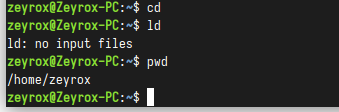
\includegraphics[width=\textwidth]{Image-TD-4/commande_test.png}
    \caption{Quelque commande pour tester HISTIGNORE}
  \end{subfigure}
  \vspace{0.9cm} % Espace verticale entre les images
  \begin{subfigure}{0.45\textwidth}
    \centering
    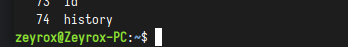
\includegraphics[width=\textwidth]{Image-TD-4/history1.png}
    \caption{Résultat dans history}
  \end{subfigure}
  \caption{Deux captures d'écran montrant un test de HISTIGNORE}
\end{figure}

\subsection{TD-5 : Alias}

\begin{itemize}
  \item Il est possible de créer des alias avec des arguments à l'aide des bash functions : 
\end{itemize}

\vspace{0.3cm}

Ecrire une bash function mkcd mondossier qui crée le dossier mondosser puis navigue dedans. 

\vspace{0.3cm}

Voici les étapes ci-dessous pour créer une bash function mkcd : 

\vspace{0.3cm}

\begin{center}
  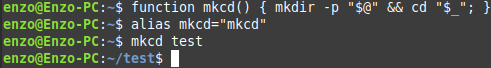
\includegraphics[width=10cm]{Image-TD-5/mkcd.png}
\end{center}

\vspace{0.3cm}

Ecrire une bash function gitemergency qui add, commit, et push tout son travail sur l'origine, permettant de ne rien perdre en cas d'alerte d'incendie.

\vspace{0.3cm}

Voici les étapes ci-dessous pour créer une bash function gitemergency : 

\vspace{0.3cm}

\begin{center}
  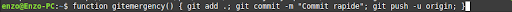
\includegraphics[width=14cm]{Image-TD-5/gitemergency.png}
\end{center}

\newpage

\subsection{TD-8 : Raccourci ZSH}

\vspace{0.3cm}

\begin{itemize}
  \item Dans zsh, créer un raccourci \texttt{Ctrl + Shift + A} :\\
  Lance les services apache et mariadb\\
  Log dans le terminal quand tout est lancé\\
  Ce reccourci est un interrupteur : apache et mariadb s'arrêtent si j'appuie à nouveau dessus.
\end{itemize}

\vspace{0.3cm}

Pour répondre à la question, nous allons tout d'abord crée un script bash comme ci-dessous : 

\vspace{0.3cm}

\begin{center}
  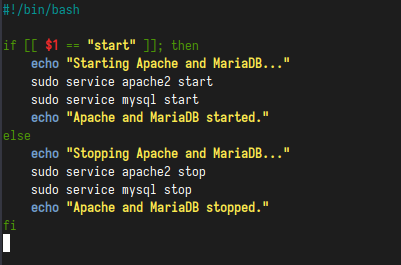
\includegraphics[width=7cm]{Image-TD-8/Sevices.png}
\end{center}

\vspace{0.3cm}

Maintenant que nous avons crée le scrpite .sh, nous allons crée deux fonctions dans le fichier .zshrc pour faire fonctionner le script comme ci-dessous : 

\vspace{0.3cm}

\begin{center}
  \includegraphics[width=7cm]{Image-TD-8/fonction\_zsh.png}
\end{center}

\vspace{0.3cm}

Maintenant que nous avons crée les deux fonctions, nous allons les combinaison de touche dans le fichier .zshrc comme ci-dessous : 

\vspace{0.3cm}

\begin{center}
  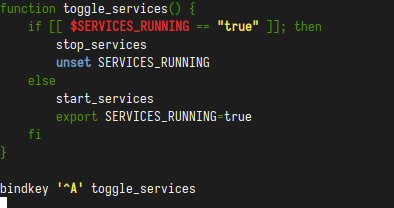
\includegraphics[width=7cm]{Image-TD-8/bindkey.png}
\end{center}

\vspace{0.3cm}

Il nous reste plus qu'à utiliser la commande \texttt{source ~/.zshrc} pour que les modification soient prises en comptes.

\newpage

  \subsection{TD-9 : Terminaux}

\vspace{0.3cm}

\begin{itemize}
  \item Installez et essayer 3+ émulateur de terminaux parmis la liste précédente : 
\end{itemize}

\vspace{0.3cm}

Pour ma part, je vais installer Terminator, Kitty et Tillix. Les installation des différantes terminaux sous debain en dessous :

\vspace{0.3cm}

Terminator : sudo apt-get install terminator

\vspace{0.3cm}

Image de Terminator : 

\vspace{0.3cm}

\begin{center}
  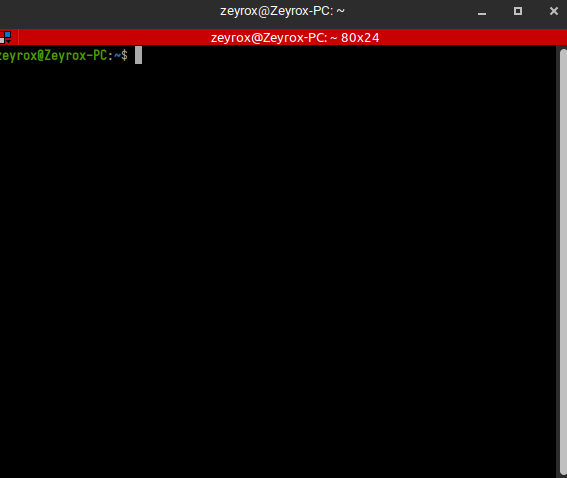
\includegraphics[width=7cm]{Image-TD-9/terminator.png}
\end{center}

\vspace{0.3cm}

Kitty: sudo apt-get install kitty

\vspace{0.3cm}

Image de Kitty : 

\vspace{0.3cm}

\begin{center}
  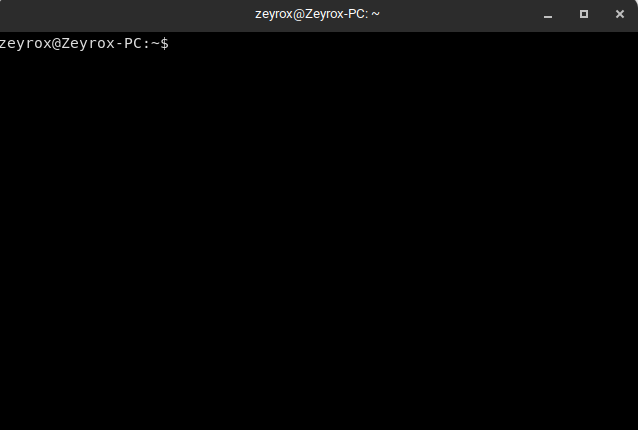
\includegraphics[width=7cm]{Image-TD-9/Kitty.png}
\end{center}

\newpage

\vspace{0.3cm}

Tilix: sudo apt-get install tilix

\vspace{0.3cm}

Image de Tilix : 

\vspace{0.3cm}

\begin{center}
  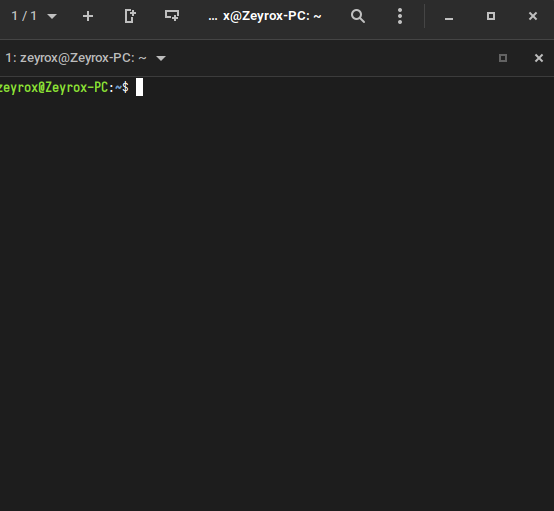
\includegraphics[width=7cm]{Image-TD-9/Tilix.png}
\end{center}

\vspace{0.3cm}

\begin{itemize}
  \item Choisir un terminal et justifier pourquoi \\
  Focntionnalitès\\
  Rapidité\\
  Documentation/Ecosystème
\end{itemize}

\vspace{0.3cm}

J'ai décidé de chosire terminator car il offre beaucoup de possibilité.
Au niveaux de la fonctionnalités, Terminator permet d'avoir plusieur terminaux dans un seul terminal (Multiplexage).
On peut crée des onglets, de définir des reccourcie et bien plus encore.

\vspace{0.3cm}

Ensuite, en ce qui concerne la rapidité, terminator est un terminal trés rapide et réactifs. 

\vspace{0.3cm}

Et pour finir, Terminator à une communauté trés actif et il est trés bien documenté. Donc on oeut conclure que dans l'ensemble, 
Terminator est un bon choix de terminal en raison de ses fonctionnalités, de sa rapidté et de sa trés bonne documentation.
C'est pour cela que j'ai décider d'utiliser Terminator. 

\vspace{0.3cm}

Et de mon point de vue, j'ai toujours utiliser terminator car je trouve qu'il est facile à utiliser et une fois que l'on connaits
les différentes combinaisons de touche, il peut devenir trés puissant.

\vspace{0.3cm}

\begin{itemize}
  \item Désinstaller les autres terminaux
\end{itemize}

\vspace{0.3cm}

Pour désinstaller les autre terminaux, nous allons utiliser la commande suivante : 

\vspace{0.3cm}

sudo apt-get remove (le nom de terminal). Par exemple : sudo apt-get remove tilix.




\newpage

\section{Client SSH}

  \subsection{TD-1-SSH : Utilisation SSH}

\begin{itemize}
  \item Récupérer et démarrer l'environnement Vagrant sur arche ?
\end{itemize}

\vspace{0.3cm}

Pour ce nouveau TD, nous allons utiliser Vagrant pour utiliser SSH. Pour ce faire, nous allons télécharger depuis Arche le fichier Vagrant. Une fois que le fichier Vagrant est téléchargé, nous allons exécuter la machine Vagrant avec la commande ci-dessous :

\vspace{0.3cm}

\begin{center}
  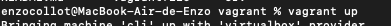
\includegraphics[width=7cm]{Image-TD-SSH-1/vagrant_up.png}
\end{center}

\vspace{0.3cm}

Une fois que la commande est terminer, on doit avoir ceci comment message qui indique que les machine sont bien démarrer : 

\vspace{0.3cm}

\begin{center}
  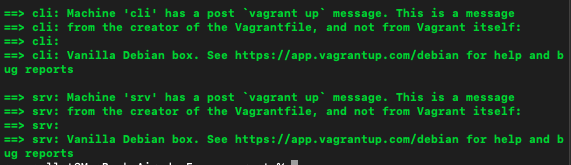
\includegraphics[width=7cm]{Image-TD-SSH-1/Machine.png}
\end{center}

\vspace{0.3cm}

\begin{itemize}
  \item Se connecter à la machine srv avec les utilisateurs alice, bob et carole sans utiliser vagrant ssh ?
\end{itemize}

\vspace{0.3cm}

Pour se connecter à la machine srv avec les utilisateurs alice, bob et carole sans utiliser vagrant ssh, nous allons utiliser la commande suivante : 

\vspace{0.3cm}

Connexion à l'utilisateur alice en ssh  : 

\vspace{0.3cm}

\begin{figure}[h]
  \centering
  \begin{subfigure}{0.30\textwidth}
    \centering
    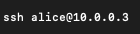
\includegraphics[width=\textwidth]{Image-TD-SSH-1/SSH-Alice.png}
    \caption{Connexion SSH avec l'utilisatrice Alice}
  \end{subfigure}
  \vspace{0.9cm} % Espace verticale entre les images
  \begin{subfigure}{0.45\textwidth}
    \centering
    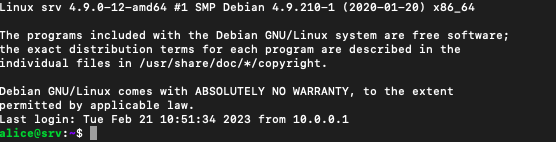
\includegraphics[width=\textwidth]{Image-TD-SSH-1/Connexion-SSH-Alice.png}
    \caption{Connexion Réussie avec l'utilisatrice Alice}
  \end{subfigure}
  \caption{Deux captures d'écran montrants une connexion en ssh au serveur srv avec l'utilisatrice Alice}
\end{figure}

\vspace{0.3cm}

Maintenant que nous avons réussi à nous connecter au serveur "srv" avec l'utilisateur "Alice", nous allons faire la même chose pour les deux autres utilisateurs.

\vspace{0.3cm}

\newpage

\vspace{0.3cm}

Connexion à l'utilisateur bob en ssh  : 

\vspace{0.3cm}

\begin{figure}[h]
  \centering
  \begin{subfigure}{0.30\textwidth}
    \centering
    
\includegraphics[width=\textwidth]{Image-TD-SSH-1/SSH-Bob.png}
    \caption{Connexion SSH avec l'utilisateur Bob}
  \end{subfigure}
  \vspace{0.9cm} % Espace verticale entre les images
  \begin{subfigure}{0.45\textwidth}
    \centering
    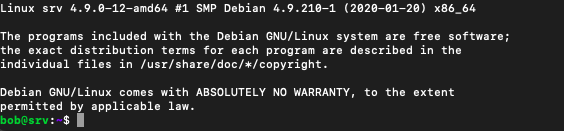
\includegraphics[width=\textwidth]{Image-TD-SSH-1/Connexion-SSH-Bob.png}
    \caption{Connexion Réussie avec l'utilisateur Bob}
  \end{subfigure}
  \caption{Deux captures d'écran montrants une connexion en ssh au serveur srv avec l'utilisateur Bob}
\end{figure}

\vspace{0.3cm}

Connexion à l'utilisateur carol en ssh  : 

\vspace{0.3cm}

\begin{figure}[h]
  \centering
  \begin{subfigure}{0.30\textwidth}
    \centering
    
\includegraphics[width=\textwidth]{Image-TD-SSH-1/SSH-Carol.png}
    \caption{Connexion SSH avec l'utilisatrice Carol}
  \end{subfigure}
  \vspace{0.9cm} % Espace verticale entre les images
  \begin{subfigure}{0.45\textwidth}
    \centering
    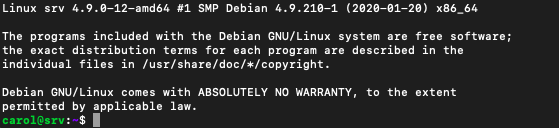
\includegraphics[width=\textwidth]{Image-TD-SSH-1/Connexion-SSH-Carol.png}
    \caption{Connexion Réussie avec l'utilisatrice Carol}
  \end{subfigure}
  \caption{Deux captures d'écran montrants une connexion en ssh au serveur srv avec l'utilisatrice Carol}
\end{figure}

\vspace{0.3cm}

\newpage

\vspace{0.3cm}

\begin{itemize}
  \item Vérifier qu'on est bien sur la machine Vagrant et pas en local ?
\end{itemize}

\vspace{0.3cm}

Pour verifier que nous somme bien sur la machine vagrant et non en local, nous allons utiliser la commande suivante : 

\vspace{0.3cm}

\begin{center}
  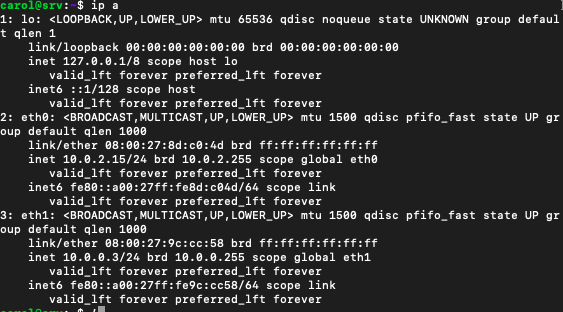
\includegraphics[width=7cm]{Image-TD-SSH-1/Commande-IPA.png}
\end{center}

\vspace{0.3cm}

On peut constater qu'au niveau des adresses IP, nous avons celle du serveur "srv", donc nous sommes bien sur la machine "vagrant".

\vspace{0.3cm}

\begin{itemize}
  \item Consulter l' history local, que remarque-t-on ?
\end{itemize}

\vspace{0.3cm}

Voici, ci-dessous l'history local : 

\vspace{0.3cm}

\begin{center}
  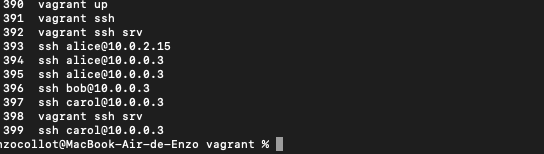
\includegraphics[width=7cm]{Image-TD-SSH-1/History-Local.png}
\end{center}

\vspace{0.3cm}

On peut constater que nous ne voyons pas les mots de passe que nous avons entrés pour nous connecter au serveur srv avec un utilisateur.


\subsection{TD-2-SSH : Authentification Publique}

\vspace{0.3cm}

\begin{itemize}
  \item Créer une paire de clés privée et publique à l'aide de ssh-keygen ?
\end{itemize}

Pour cette nouvelle étape, nous allons créer une paire de clés privée et publique à l'aide de ssh-keygen. Donc voici les étape ci-dessous pour le faire : 

\vspace{0.3cm}

Pour commencer, nous allons ouvrie un terminal est taper la commande suivante  : 

\vspace{0.3cm}

\begin{center}
  
\includegraphics[width=7cm]{Image-TD-SSH-2/ssh-keygen.png}
\end{center}

\vspace{0.3cm}

Ensuite, il nous demande à quel emplacement nous voulons enregistrer notre clé. Nous laissons par défaut :

\vspace{0.3cm}

\begin{center}
  
\includegraphics[width=7cm]{Image-TD-SSH-2/Emplacement-cle.png}
\end{center}

\vspace{0.3cm}

\newpage


Ensuite, il nous demande une passphrase. Vous pouvez en indiquer une, mais j'ai laissé par défaut. Une fois que c'est fini, vous devez avoir cela qui devrait apparaître :

\vspace{0.3cm}

\begin{center}
  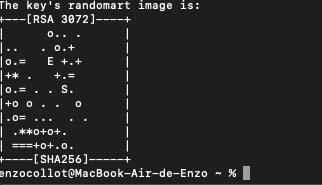
\includegraphics[width=7cm]{Image-TD-SSH-2/Génération-cle.png}
\end{center}

\vspace{0.3cm}

Voila, nous avons générer une clé rsa.

\vspace{0.3cm}

\begin{itemize}
  \item Utiliser la commande ssh-copy-id pour déposer la clé publique sur le compte alice@cli . Vérifier qu'on peut maintenant se connecter sans mot de passe ?
\end{itemize}

\vspace{0.3cm}

Pour cette nouvelle étape, nous allons utiliser la commande ssh-copy-id pour déposer la clé publique sur le compte alice@cli. Pour ce faire, nous allons utiliser la commande suivantes : 

\vspace{0.3cm}

\begin{center}
  
\includegraphics[width=7cm]{Image-TD-SSH-2/ssh-copy-id.png}
\end{center}

\vspace{0.3cm}

Une fois que nous avons entrée la commande, il va nous demander le mot de passe de Alice. Une fois le mots de passe entrer, nous avons ceci qui apparaît : 

\vspace{0.3cm}

\begin{center}
  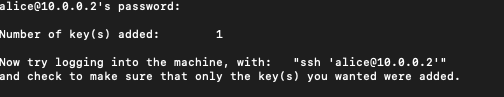
\includegraphics[width=7cm]{Image-TD-SSH-2/key-add.png}
\end{center}

\vspace{0.3cm}

Maintenant, on peut ce connecter en compte d'alice sur le serveur cli sans rentrer son mots de passe.

\vspace{0.3cm}

\begin{itemize}
  \item Déposer manuellement la clé publique sur le compte bob@cli \\
  Les nouvelles clés créés sont dans ~/.ssh\\
  Les clées autorisées à se connecter au serveur sont dans ~/.ssh/authorized\_keys
\end{itemize}

\vspace{0.3cm}

Pour déposer manuellement la clé publique sur le compte bob@cli, vous pouvez suivre les étapes ci-dessous : 

\vspace{0.3cm}

Pour commencer, nous allons afficher le contenue de notre clé publique et le copier avec la commande suivante : 

\vspace{0.3cm}

\begin{center}
  \includegraphics[width=7cm]{Image-TD-SSH-2/Clé-pub.png}
\end{center}

\vspace{0.3cm}

\newpage

Une fois que nous avons copier la clé publique, nous allons nous connecter au compte de bob@cli avec la commande suivante : \\

\texttt{ssh bob@cli}

\vspace{0.3cm}

Une fois connecter sur le compte, nous allons verifier si le dossier .ssh existe. Si il existe pas, nous le créons avec la commande suivante : \\

\texttt{mkdir ~/.ssh}

\vspace{0.3cm}

Ensuite, on tape la commande suivante pour créer ou ouvrir le fichier "authorized\_keys" : \\

\texttt{nano ~/.ssh/authorized\_keys}

\vspace{0.3cm}

Maintenant, on copie le contenue de la clé publique dans le fichier comme ci-dessous  : 

\vspace{0.3cm}

\begin{center}
  \includegraphics[width=7cm]{Image-TD-SSH-2/clé-pub-bob.png}
\end{center}

\vspace{0.3cm}

Une fois que nous avons enregistrer le fichier, c'est bon, on peut ce connecter au compte de bob@cli sans taper le mot de passe avec la commande suivante : \\  

\texttt{ssh -i ~/.ssh/id\_rsa.pub bob@cli}


\subsection{TD-3-SSH : Connexion Automatique}

\begin{itemize}
  \item Purger le fichier ~/.ssh/known\_hosts si nécessaire ?
\end{itemize}

\vspace{0.3cm}

Pour cette nouvelle étape, nous allons purger le fichier ~/.ssh/known\_hosts avec la commande suivante : 

\texttt{sudo rm known\_host}

\vspace{0.3cm}

\begin{itemize}
  \item A l'aide de ssh-keygen et ssh-keyscan , ajouter la clé publique du serveur srv manuellement, décrire les étapes. \\
  Votre client SSH ne doit pas demander d'ajouter la clé publique du serveur à la première connexion.
\end{itemize}

\vspace{0.3cm}

Voici les étapes pour ajouter manuellement la clé publique du serveur srv au fichier known\_hosts à l'aide des commandes ssh-keygen et ssh-keyscan :

\vspace{0.3cm}

Tout d'abord, on va utiliser la commande ssh-keyscan pour récupérer la clé publique du serveur srv. Dans un terminal, on va utiliser la commande suivante : 

\texttt{ssh-keyscan 10.0.0.3 >> ~/.ssh/known\_hosts}

\vspace{0.3cm}

\begin{center}
  
\includegraphics[width=7cm]{Image-TD-SSH-3/ssh-keyscan.png}
\end{center}

\vspace{0.3cm}

\begin{center}
  \includegraphics[width=7cm]{Image-TD-SSH-3/résultat-ssh-keyscan.png}
\end{center}

\vspace{0.3cm}

\newpage

Ensuite, on va utiliser la commande ssh-keygen pour générer une paire de clés SSH (une clé publique et une clé privée) sur l'ordinateur local. Dans le même terminal, tapez la commande suivante :

\texttt{ssh-keygen}

\vspace{0.3cm}

\begin{center}
  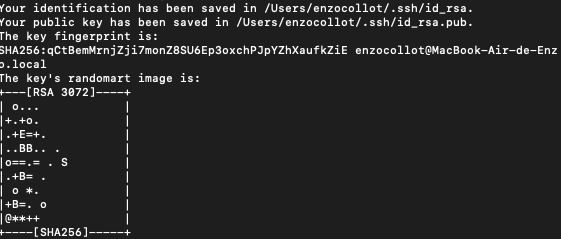
\includegraphics[width=7cm]{Image-TD-SSH-3/Génération-key.png}
\end{center}


\vspace{0.3cm}

Une fois que nous avons généré une paire de clés SSH, nous allons  copier la clé publique sur le serveur srv. Pour ce faire, nous allons entrer la commande suivante dans le terminal :

\texttt{ssh-copy-id -i ~/.ssh/id/\_rsa.pub user@srv} 

\vspace{0.3cm}

Ici, user@srv on remplace par les utilisateur sur le serveur srv. un petit exemple ci-dessous  : 

\vspace{0.3cm}

\begin{center}
  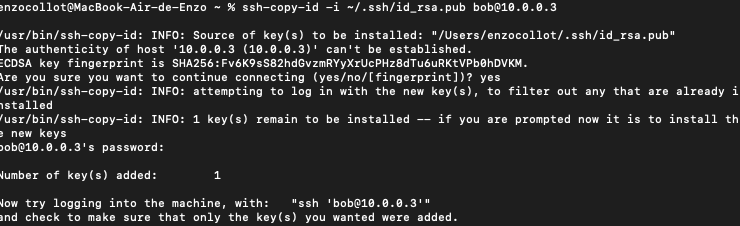
\includegraphics[width=7cm]{Image-TD-SSH-3/ssh-copy-id.png}
\end{center}

\vspace{0.3cm}

Voila, maintenant, on peut se connecter automatique avec l'utilisateur bob au serveur srv.

\vspace{0.3cm}

\begin{itemize}
  \item Créer un fichier de configuration pour SSH, vous permettant de vous connecter sur le compte bob@cli en tapant ssh bc.
\end{itemize}

\vspace{0.3cm}

Voici les étapes pour créer un fichier de configuration pour SSH qui permettra de se connecter au compte bob@cli en tapant simplement ssh bc :

\vspace{0.3cm}

Pour commencer, nous allons tapez la commande suivante pour créer un nouveau fichier de configuration SSH :

\texttt{nano ~/.ssh/config}

\vspace{0.3cm}

\begin{center}
  
\includegraphics[width=7cm]{Image-TD-SSH-3/fichier-config.png}
\end{center}

\vspace{0.3cm}

Dans le fichier de configuration, ajoutez les lignes suivantes :

\vspace{0.3cm}

\begin{center}
  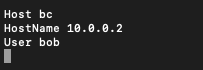
\includegraphics[width=7cm]{Image-TD-SSH-3/ligne-conf.png}
\end{center}

\vspace{0.3cm}

\newpage

Une fois que nous avons mis les informations dans le fichier de configuration, nous pouvons nous connecter comme ci-dessous : 

\vspace{0.3cm}

\begin{figure}[h]
  \centering
  \begin{subfigure}{0.30\textwidth}
    \centering
    \includegraphics[width=\textwidth]{Image-TD-SSH-3/Connexion-SSH-Complétion.png}
    \caption{Connexion SSH en utilisant l'auto-complétion}
  \end{subfigure}
  \vspace{0.9cm} % Espace verticale entre les images
  \begin{subfigure}{0.45\textwidth}
    \centering
    \includegraphics[width=\textwidth]{Image-TD-SSH-3/Connexion-réussite.png}
    \caption{Connexion réussite avec l'utilisateur Bob}
  \end{subfigure}
  \caption{Deux captures d'écran montrants une connexion en ssh au serveur srv avec l'utilisateur bob en utilisant l'auto-complétion}
\end{figure}

\vspace{0.3cm}

\begin{itemize}
  \item Vérifiez que vous arrivez à vous connecter au compte alice@cli en utilisant SFTP. \\ 
  Copiez-y un fichier par SFTP, puis récupérez un autre fichier. ?
\end{itemize}

\vspace{0.3cm}

Pour cette nouvelle étape, nous allons nous connecter avec l'utilisateur alice en utilisant SFTP. Pour ce faire, nous allons ouvrir un terminal et taper la commande suivante : 

\texttt{sftp alice@10.0.0.2}

\vspace{0.3cm}

\begin{center}
  
\includegraphics[width=7cm]{Image-TD-SSH-4/commande-sftp.png}
\end{center}

\vspace{0.3cm}

\begin{center}
  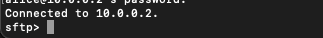
\includegraphics[width=7cm]{Image-TD-SSH-4/connexion-sftp.png}
\end{center}

\vspace{0.3cm}

On peut constater que nous somme bien connecter en sftp au serveur cli avec l'utilisateur Alice.

\vspace{0.3cm}

Maintenant que nous somme connecté, nous allons copier un fichier de notre machine local vers la machine virutel. Pour ce faire, nous allons crée un fichier texte et l'envoyer sur le serveur. Voici les étapes ci-dessous : 

\vspace{0.3cm}

Pour commencer, nous allons crée un fichier texte avec la commande suivante  : 

\vspace{0.3cm}

\begin{center}
  \includegraphics[width=7cm]{Image-TD-SSH-4/création-fichier.png}
\end{center}

\vspace{0.3cm}

Une fois que nous avons crée le fichier, on se reconnecte un serveur avec la commande que nous avons vue précédement. Une fois connecter, nous allons utiliser la commande suivante : 

\vspace{0.3cm}

\begin{center}
  
\includegraphics[width=7cm]{Image-TD-SSH-4/fichier-envoyer.png}
\end{center}

\vspace{0.3cm}

\begin{center}
  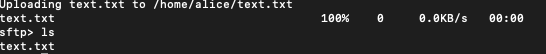
\includegraphics[width=7cm]{Image-TD-SSH-4/commande-reussite.png}
\end{center}

\vspace{0.3cm}

On peut constater que notre fichier à bien était envoyé sur le serveur. 

\vspace{0.3cm}

Maintenant que nous avons envoyer un fichier de notre machine local vers la machine virtuelle, nous allons prendre un fichier de la machine virtuelle et nous allons le télécherger sur la machine local. Pour ce faire, nous allons utiliser la commande suivante : 

\vspace{0.3cm}

\begin{center}
  
\includegraphics[width=7cm]{Image-TD-SSH-4/commande-puts.png}
\end{center}

\vspace{0.3cm}

\begin{center}
  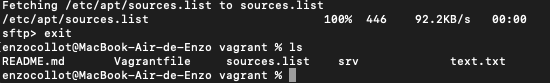
\includegraphics[width=7cm]{Image-TD-SSH-4/commande-puts-2.png}
\end{center}

\vspace{0.3cm}

On peut constater que nous avons bien reçus le fichier du serveur sur notre machine local.

\vspace{0.3cm}

\begin{itemize}
  \item Vérifiez que vous arrivez à vous connecter au compte alice@cli avec SSHFS. \\
  Éditez un fichier distant avec un éditeur graphique (par exemple GVIM)
\end{itemize}

\vspace{0.3cm}

\begin{itemize}
    \item Vérifiez que la modification est bien répercutée sur la machine virtuelle alice@cli.
\end{itemize}

\vspace{0.3cm}

Pour cette nouvelle étape, je vais répondre au deux question en même temps. Pour commencer, nous allons nous connecter au compte alice&cli avec SSHFS. Pour ce faire, nous allons utiliser la commande suivante : 

\vspace{0.3cm}

\begin{center}
  \includegraphics[width=7cm]{Image-TD-SSH-4/sshfs.png}
\end{center}

\vspace{0.3cm}

Verfication du montage dans le dossier /tmp/alicli : 

\vspace{0.3cm}

\begin{center}
  \includegraphics[width=7cm]{Image-TD-SSH-4/montage-sshfs.png}
\end{center}

\vspace{0.3cm}

On peut constater que le montage à bien était réalisé. 

\vspace{0.3cm}

Maintenant, nous allons modifier un fichier avec vim et regarder si les modification se repercute quand on se connecte directement au serveur. Pour ce faire, nous allons créé un fichier avec vim et mettre des informations dedans comme ci-dessous  : 

\vspace{0.3cm}

\begin{center}
  \includegraphics[width=7cm]{Image-TD-SSH-4/Modification-fichier-vim.png}
\end{center}

\vspace{0.3cm}

Une fois que nous avons créé et modifié le fichier, nous allons nous connecter au serveur avec alice comme ci-dessous : 

\vspace{0.3cm}

\begin{center}
  \includegraphics[width=7cm]{Image-TD-SSH-4/connexion-ssh.png}
\end{center}

\vspace{0.3cm}

Une fois que nous somme connecter, nous allons regarder les information dans le fichier comme ci-dessous  : 


\vspace{0.3cm}

\begin{center}
  \includegraphics[width=7cm]{Image-TD-SSH-4/verfication-fichier.png}
\end{center}

\vspace{0.3cm}

On peut constater que notre fichier à bien était modifier.

\end{document}